\documentclass[11pt]{article}
\usepackage{setspace}
\setstretch{1}
\usepackage{amsmath,amssymb, amsthm}
\usepackage{graphicx}
\usepackage{bm}
\usepackage[hang, flushmargin]{footmisc}
\usepackage[colorlinks=true]{hyperref}
\usepackage[nameinlink]{cleveref}
\usepackage{footnotebackref}
\usepackage{url}
\usepackage{listings}
\usepackage[most]{tcolorbox}
\usepackage{inconsolata}
\usepackage[papersize={8.5in,11in}, margin=1in]{geometry}
\usepackage{float}
\usepackage{caption}
\usepackage{esint}
\usepackage{url}
\usepackage{enumitem}
\usepackage{subfig}
\usepackage{wasysym}
\newcommand{\ilc}{\texttt}
\usepackage{etoolbox}
\usepackage{algorithm}
\usepackage{changepage}
% \usepackage{algorithmic}
\usepackage[noend]{algpseudocode}
\usepackage{tikz}
\usetikzlibrary{matrix,positioning,arrows.meta,arrows}
\patchcmd{\thebibliography}{\section*{\refname}}{}{}{}
% \PassOptionsToPackage{hyphens}{url}\usepackage{hyperref}

\providecommand{\myceil}[1]{\left \lceil #1 \right \rceil }
\providecommand{\myfloor}[1]{\left \lfloor #1 \right \rfloor }


\begin{document}



\title{\textbf{CSDS 455: Homework 20}}

\author{Shaochen (Henry) ZHONG, \ilc{sxz517}}
\date{Due and submitted on 11/02/2020 \\ Fall 2020, Dr. Connamacher}
\maketitle

\textit{I have consulted Yige Sun and Yuhui Zhang for the following problems.}

\section*{Problem 1}

\textit{I have consulted and cited visual aids from \url{https://cseweb.ucsd.edu/classes/sp11/cse202-a/lecture7-final.pdf}.}

Let \ilc{I(u)} to be the maximum independent set of the subtree rooted to node \ilc{u}. We will have two cases:


\begin{figure}[H]
    \centering
    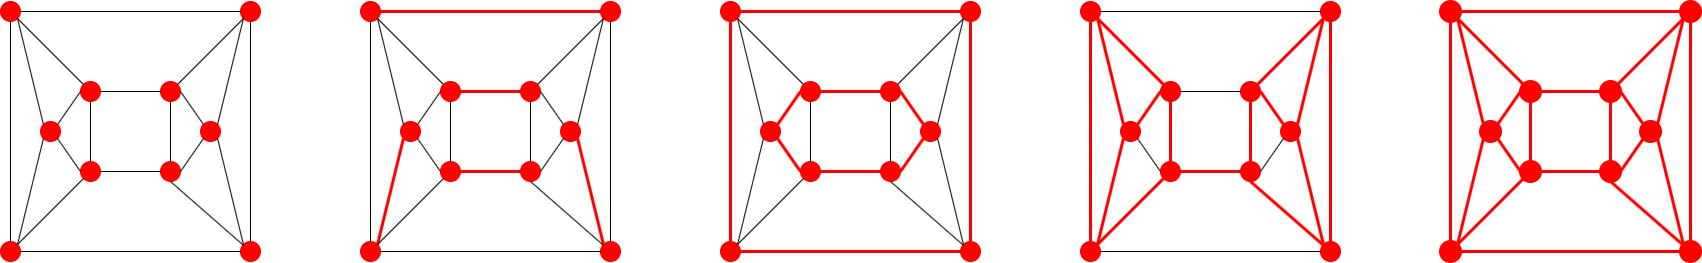
\includegraphics[width=0.4\linewidth]{{fig/fig_p1.png}}
\end{figure}

\begin{itemize}
    \item \ilc{I(u)} includes \ilc{u}.
    \item \ilc{I(u)} does not \ilc{u}, but includes children of \ilc{u}.
\end{itemize}


\noindent Since the goal is to maximize the size of the set, we have \ilc{I(u)} to be:

\begin{equation*}
    I(u) = \max \{\sum_{\text{child $v$ of $u$}} I(v), \ \  1 + \sum_{\text{grandchild $w$ of $u$}} I(w)\}
\end{equation*}

Then we may simply do a postorder traversal from leaves to the root of the tree, the runtime will therefore be $O(|T|)$.

\section*{Problem 2}

We will try to make $T$ a tree composition out of $k$-tree $T_k$. We first identify all the verticies with degree $k$, add them as leaves of $T$; we call them the ``first group''. Then we update $G$ by removing all the vertices and edges of vertices in $T$, and find the next (second) group of verticies with degree $k$ -- if two verticies out of the two (different) groups has an edge connected to them, they are child-parent (according to the order of deletion) in $T$. We may do this procedure recursively until we are left with a $k$ or $k+1$ clique, which will be the root of $T$.\newline

We know that $T$ will be a tree, as no vertices with degree $k$ is connected to more than one vertex with degree $k$ with all verticies of the first group removed (namely, no verticies in the ``first group'' is connected to two verticies in the ``second group''). This procedure may potentialy take $O(|T_k| \cdot k)$ as we have to evaluate almost every verticies in $T_k$ meanwhile each of the verticies has $k$ potential ``parent'' to evaluate with.

We then run the algorithm introduced in \textit{Problem 1} on $T$, which will take $O(|T|)$ time which will be absorbed to $O(|T_k| \cdot k)$.


\section*{Problem 3}

\textit{I have consulted \url{https://en.wikipedia.org/wiki/Tree_decomposition}.}

Let $T$ be the tree composition of $G$ with treewith $k$. We denote $X_i$ to be a node (bag) of $T$ and $X_j$ to be one of the child nodes of $X_i$ (if we traverse $T$ from an arbitary root). Let $S \subset X_i$ and $S' \subset (X_i \cap X_j)$, we further denote:

\begin{itemize}
    \item $A(S, i)$ to be the largest independent set $I$ among all $X_j$ such that $I \cap X_i = S$.
    \item $B(S', i, j)$ to be the largest independent set $I$ among all $X_j$ such that $I \cap X_i \cap X_j = S'$.
\end{itemize}

We have the DP structure of (starts from a leave of tree $T$):

\begin{align*}
    A(S, i) &= S + \sum_{j} (B (S \cap X_j, i, j) - S \cap X_j) \\
    B(S, j, i) &= \max(|A(S', i)|) \ \Big\mid \ \text{for} \ S' \subset X_j, S = S' \cap X_i
\end{align*}

The algorithm works because if we want $S \subset X_i$ to be part of the maximum independent set $M$ of $G$, then we need to find all of the verticies that are independent to $S$ to add to $M$ -- from a DP standpoint, we will need to find how many vertices in the child nodes of $X_i$ can be add to $M$ along with $S$. $B (S \cap X_j, i, j)$ is an independent set $I'$ where $I' \cap X_i \cap X_j = S \cap X_j$. This means $I'$ can be add to $M$ along with $S$ as nothing in $I'$ is connected to $S \cap X_j$ since $S \cap X_j$ is in $I'$, and nothing in $I'$ is connected to $S - S \cap X_j$ since $S - S \cap X_j$ are in $X_i$ but not in $X_j$, and $I'$ was exclusively selected from $X_j$. The only problem is $I'$ will be double-counting $S \cap X_j$ which already added to $A(S, i)$ with the leading $S$, so we remove them.

By doing this recursively on all $X_j$, we may find the $M$ with respect to $S$.\newline

The runtime of calculating this $M$ is $O(|j|k)$ as we need $O(k)$ to figure out if the picked $S$ is an independent set, and there are $|j|$ children of $X_i$ to run the above algorithm with. Which is $\approx O(|G|)$ as we know that $|j|$ is at most $|T| - 1$ and $O((|T| - 1) k) < O(|G|)$.\newline

Now we still need to find the best $S$ for $X_i$. Since $|X_i| \leq k + 1$, there are $2^{k+1} \approx 2^k$ subsets to consider. Combine the runtime of the procedure above together, we have $O(2^k|G|)$.

\end{document}